\section{Results}
We analyze the \nSplitZero{} validation questions of CRAG Task~1\&2. Under our
string-grounding procedure, \nGroundPct{} of questions are \emph{groundable} (the
gold answer appears verbatim in the retrieved pages); the remainder---dominated by
false-premise items and answers that never occur as a literal span (many
aggregation and dynamic questions)---are excluded from sufficiency statistics. At
$k{=}3$, BM25 surfaces the gold passage in the top-$k$ at some prefix for
\nRetrPct{} of all questions. All reported $\phi_{\mathrm{suf}}$ statistics are
conditional on this retrieved-gold population; $\phi_{\mathrm{sc}}$ is defined for
every question and serves as a grounding-free check.

\subsection{RQ1: How is stabilization distributed?}
The two stabilization notions behave very differently (Fig.~\ref{fig:phi}).
Self-consistency stabilizes \emph{late}: the lexical top-1 keeps changing until,
on average, $\phi_{\mathrm{sc}}$ reaches mean \phiScMean{} (median \phiScMed{})---
roughly three-quarters of the way through the query. Sufficiency, in contrast,
stabilizes \emph{early}: the gold passage enters the top-$k$ at mean
$\phi_{\mathrm{suf}}=\phiSufMean{}$ and median \phiSufMed{}. The gap is the central
empirical observation of this study: \textbf{the answer-bearing document is
retrievable from a short prefix long before the query's lexical top-1 settles}.
For streaming tool use this is the favorable regime---one need not wait for the
utterance to ``finish'' for the right evidence to be in hand.

The $\phi_{\mathrm{suf}}$ distribution (Fig.~\ref{fig:phi}) is right-skewed with a
large mass near zero and a thinner late tail, rather than cleanly bimodal as
H1 anticipated. Volatility is modest: the post-stabilization top-1 changes at all
for only \volSharePct{} of questions (mean $V=\volMean{}$), so early-commit risk is
concentrated in a minority of queries rather than pervasive.

\begin{figure}[t]
\centering
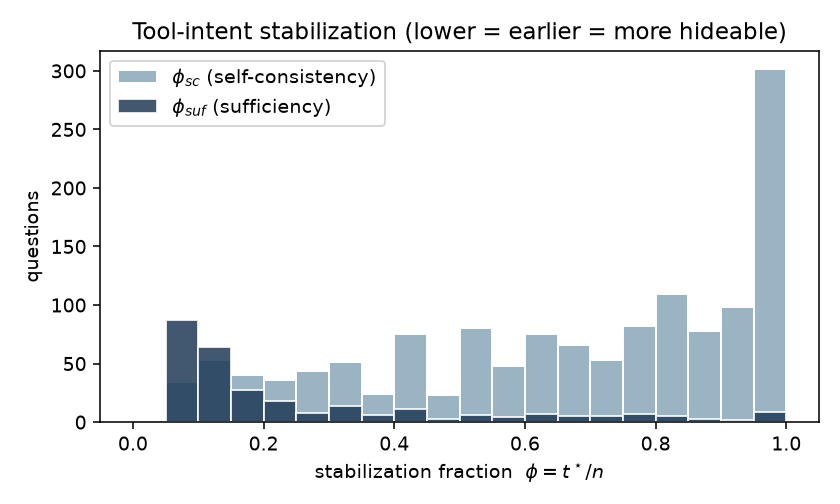
\includegraphics[width=0.78\linewidth]{figures/phi_distribution.png}
\caption{Distribution of stabilization fraction $\phi$ at $k{=}3$. Sufficiency
($\phi_{\mathrm{suf}}$, dark) concentrates near zero---gold evidence is retrievable
early---while self-consistency ($\phi_{\mathrm{sc}}$, light) is late and broad.}
\label{fig:phi}
\end{figure}

\subsection{RQ4: What predicts early vs.\ late stabilization?}
Question type is a strong predictor of $\phi_{\mathrm{suf}}$, spanning a wide range
(Table~\ref{tab:bytype}, Fig.~\ref{fig:bytype}). However, the ordering refines
hypothesis H3 rather than confirming it. H3 expected simple lookups to stabilize
early and aggregation/comparison/multi-hop to stabilize late. We instead find
\emph{aggregation} and \emph{comparison} among the \emph{earliest}-stabilizing
types, with \emph{set} questions latest. The explanation is that sufficiency
measures when the gold \emph{document} becomes retrievable, not when the answer can
be \emph{computed}: a comparison or aggregation question often names its key
entities up front, so the answer-bearing page is retrievable early even though
producing the final answer requires post-retrieval reasoning. In other words,
retrieval-sufficiency stabilization is governed by entity position in the
utterance, which is not aligned with reasoning complexity. (Several types have
small support---\texttt{set} $n{=}2$, \texttt{post-processing} $n{=}5$---so their
point estimates are noisy; the larger classes \texttt{simple}, \texttt{comparison},
and \texttt{simple\_w\_condition} are well populated.)

\begin{table}[t]
\centering
\caption{Sufficiency stabilization by CRAG question type ($k{=}3$, retrieved-gold
questions), sorted earliest to latest.}
\label{tab:bytype}
\begin{tabular}{lrr}
\toprule
question type & $n$ & mean $\phi_{\mathrm{suf}}$ \\
\midrule
aggregation          & 32  & 0.198 \\
comparison           & 59  & 0.210 \\
multi-hop            & 15  & 0.267 \\
simple               & 118 & 0.280 \\
false\_premise       & 9   & 0.289 \\
simple\_w\_condition & 52  & 0.307 \\
post-processing      & 5   & 0.310 \\
set                  & 2   & 0.658 \\
\bottomrule
\end{tabular}
\end{table}

\begin{figure}[t]
\centering
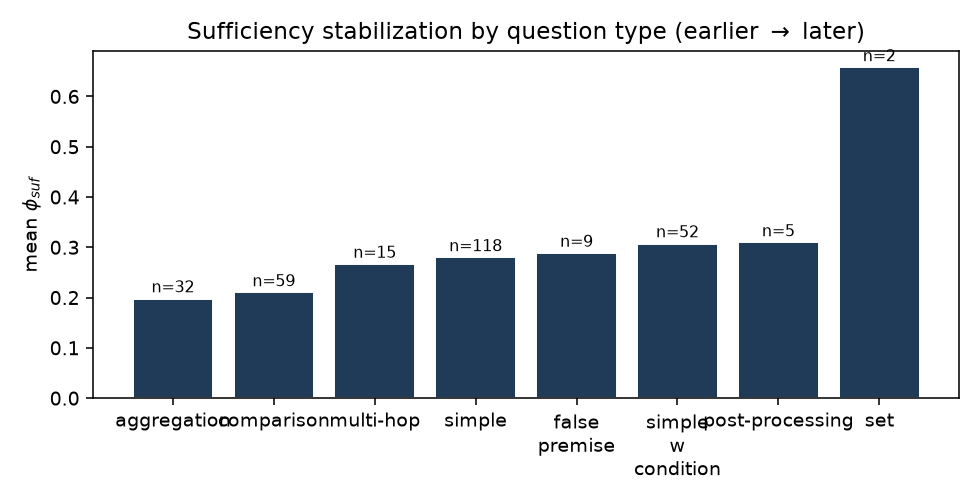
\includegraphics[width=0.92\linewidth]{figures/phi_by_type.png}
\caption{Mean $\phi_{\mathrm{suf}}$ by question type ($k{=}3$). Type spans a $3\times$
range, but the ordering tracks entity position, not reasoning complexity.}
\label{fig:bytype}
\end{figure}

\subsection{RQ2: What fraction of queries admit latency hiding?}
Using $t^\star=t_{\mathrm{suf}}$ where available and falling back to
$t_{\mathrm{sc}}$ otherwise, we compute the streamable fraction over the full
$(L,\delta,\theta)$ grid (Table~\ref{tab:rq2}, Fig.~\ref{fig:rq2}). At the central
operating point ($L{=}600$\,ms, $\delta{=}3$\,w/s, $\theta{=}0.8$), \streamPct{} of
queries admit hiding at least 80\% of tool latency. Two patterns stand out. First,
for small tool latency ($L\le300$\,ms) the constraint is essentially never binding:
$82.6\%$ of queries are streamable regardless of cadence---the residual input time
trivially covers a short tool call. Second, and confirming \textbf{H2}, when tool
latency is large ($L{=}1000$\,ms) the binding constraint becomes residual input
time, so a \emph{slower} cadence \emph{raises} the streamable fraction: from
$54.5\%$ at $\delta{=}4$\,w/s up to $73.9\%$ at $\delta{=}2$\,w/s. Faster typists
and faster talkers leave less room to hide a slow tool.

\begin{table}[t]
\centering
\caption{RQ2: streamable fraction (\%) at $\theta{=}0.8$ over the $(L,\delta)$ grid.
Rows are tool latency $L$ (ms); columns are input cadence $\delta$ (words/sec).
For large $L$, slower cadence (lower $\delta$) hides more (H2).}
\label{tab:rq2}
\begin{tabular}{lccc}
\toprule
 & $\delta{=}2$ & $\delta{=}3$ & $\delta{=}4$ \\
\midrule
$L{=}100$  & 82.6 & 82.6 & 82.6 \\
$L{=}300$  & 82.6 & 82.6 & 82.6 \\
$L{=}600$  & 82.6 & 73.9 & 73.9 \\
$L{=}1000$ & 73.9 & 63.3 & 54.5 \\
\bottomrule
\end{tabular}
\end{table}

\begin{figure}[t]
\centering
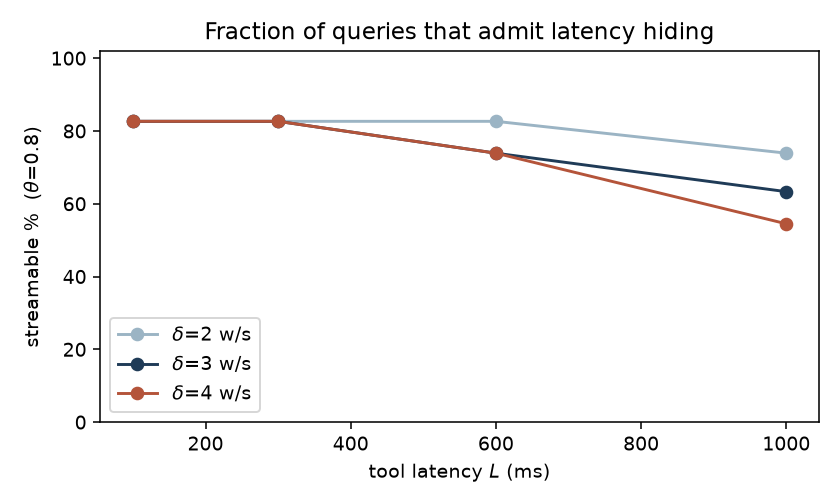
\includegraphics[width=0.78\linewidth]{figures/rq2_surface.png}
\caption{Streamable fraction vs.\ tool latency $L$ at $\theta{=}0.8$, one line per
cadence $\delta$. The curves separate only once $L$ is large enough for residual
input time to bind; there, slower cadence dominates (H2).}
\label{fig:rq2}
\end{figure}

\subsection{RQ3: Does the bound match a working pipeline?}
We replayed \rqThreeN{} retrieved-gold questions through the asynchronous Streaming
RAG harness at $L{=}600$\,ms, $\delta{=}3$\,w/s. The measured perceived-latency
saving (baseline minus streaming) averages \measSaved{}\,ms, while the $H$ bound
predicts \hPred{}\,ms (Fig.~\ref{fig:rq3}). On average, measured savings
\emph{exceed} the bound by roughly $1.9\times$ (a small number of queries where the
speculative trigger mis-fires save nothing or slightly less than baseline). This is
expected and informative:
$H$ models only the tool latency hidden behind input, whereas the calibrated
pipeline additionally overlaps the LLM's query-generation step
($\approx590$\,ms~\cite{arora2025streamrag}) with the user's input. $H$ is
therefore a \emph{conservative} predictor of realized savings---it captures the
input-hiding component and omits other overlappable costs---so a query that $H$
deems streamable will, in practice, save at least as much as predicted.

\begin{figure}[t]
\centering
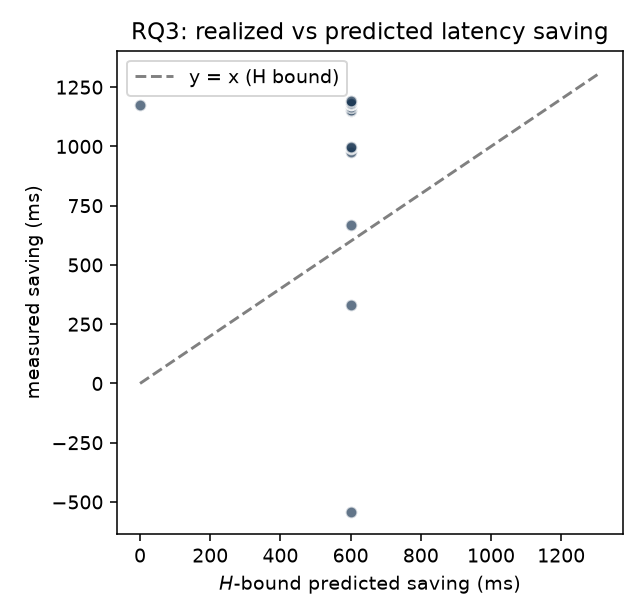
\includegraphics[width=0.5\linewidth]{figures/rq3_scatter.png}
\caption{RQ3: per-question measured saving vs.\ the $H$ bound ($\rqThreeN{}$
questions). Most points lie above $y{=}x$ because the pipeline also hides
query-generation latency, which $H$ does not model; a few queries where
speculation mis-fires show small negative savings.}
\label{fig:rq3}
\end{figure}

\subsection{Retriever robustness (top-$k$)}
Varying the sufficiency top-$k$ shifts absolute values but preserves the
qualitative picture (Table~\ref{tab:topk}). Larger $k$ surfaces the gold passage
for more questions (retrieved-gold rate $15.6\%\to25.0\%$) and stabilizes slightly
earlier (mean $\phi_{\mathrm{suf}}$ $0.327\to0.248$), as expected since a more
permissive top-$k$ is easier to satisfy. The self-consistency curve is unchanged by
$k$ (it depends only on the top-1), and the central streamable fraction is stable
near $73\text{--}74\%$. The early-sufficiency / late-self-consistency gap holds at
every $k$.

\begin{table}[t]
\centering
\caption{Top-$k$ robustness. $\phi_{\mathrm{sc}}$ (mean 0.67 / median 0.73) is
independent of $k$ and omitted.}
\label{tab:topk}
\begin{tabular}{lrrr}
\toprule
$k$ & retrieved-gold & mean $\phi_{\mathrm{suf}}$ & median $\phi_{\mathrm{suf}}$ \\
\midrule
1 & 15.6\% & 0.327 & 0.200 \\
3 & 21.3\% & 0.264 & 0.143 \\
5 & 25.0\% & 0.248 & 0.125 \\
\bottomrule
\end{tabular}
\end{table}
